\chapter{Preliminaries}
\label{chap:preliminaries}
This chapter serves as a general introduction to some mathematical concepts that are of interest to us.
\section{Graph theory}

\subsection{Basic Notation}
Let $G$ be a simple, undirected graph with vertex set $V(G)$ and edge set $E(G)$. The \textit{neighbourhood} of a vertex $v$ is denoted by
$N_{G}(v) = \{u | uv \in E(G)\}$. The \textit{degree} of a vertex $v \in G$, denoted by $deg_{G}(v)$, is $|N_{G}(v)|$. Then
$\Delta(G) = max_{v \in V(G)} deg_{G}(v)$ and $\delta(G) = min_{v \in V(G)} deg_{G}(v) $ is the maximum and minimum degree of $G$, respectively.
A subgraph of $G$ is a graph $G^{'}$ such that $V(G^{'}) \subseteq V(G)$ and $E(G^{'}) \subseteq E(G)$ (see Fig.~\ref{fig:subgraph}).

A \textit{walk} of length $l$ from $v_0$ to $v_l$ in $G$ is a vertex sequence $v_0, \dots ,v_{l}$, such that for all
$i \in \{0,\dots,l-1\}$, $v_{i}v_{i+1} \in E(G)$. It is a path if all vertices are distinct. A path from a vertex $u$ to a vertex $v$ is also
called a \textit{$uv-$path}. A graph $G$ is \textit{connected} if there is a path between every pair of vertices. The \textit{$k$-th power} of
a graph $G = (V,E)$ is the graph $G^{k}$ whose vertex set is $V$ and two distinct vertices $u,v$ are adjacent in $G^{k}$ if and only if the
shortest path distance between $u$ and $v$ in $G$ is at most $k$.
A \textit{hypergraph} $H$ is a pair $H = (X,E)$ where $X$ is a set of elements, called nodes or vertices, and $E$ is a set of non-empty subsets of $X$
called \textit{hyperedges} or \textit{links}.

An \textit{independent set} of a graph $G$ is a vextex-subset of $G$ in which
no two vertices are adjacent. Given a set of elements $\{1,2,\dots,n\}$ (called the universe, denoted $\mathcal{U}$) and a
collection $\mathcal{S}$ of $m$ sets whose union equals the universe, an \textit{exact cover} is a sub-collection $\mathcal{S}^{*}$ of $\mathcal{S}$
such that each element in $\mathcal{U}$ is contained in exactly one subset in $\mathcal{S}^{*}$. The set $\mathcal{S}$ of subsets of $U$ can be
considered as a hypergraph $H = (U, \mathcal{S})$, where each element of $U$ is a vertex and each element of $\mathcal{S}$ is a hyperedge.


For an in-depth review of general graph theoretic definitions, the reader can refer to Diestel's textbook \cite{diestel_graph_2000}.
%%%%%%%%%%%%%%%%%%%%%%%%%%%%%%%%%%%%%%%%%%%%%%%% BEGINING OF A FIGURE %%%%%%%%%%%%%%%%%%%%%%%%%%%%%%%%%%%%%%%%%%%%%%%
\begin{figure} [H]
    \centering
    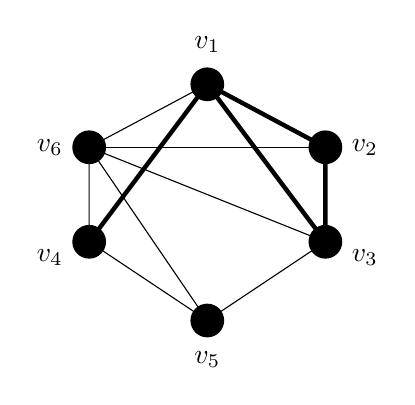
\begin{tikzpicture}
        \def\xa{1}
        \def\ya{5}
        %nodes
        \draw[thick, fill=black] (\xa,\ya) circle (0.2cm);         % v5
        \draw[thick, fill=black] (\xa+1.5,\ya+1) circle (0.2cm);   % v3
        \draw[thick, fill=black] (\xa+1.5,\ya+2.2) circle (0.2cm); % v2
        \draw[thick, fill=black] (\xa,\ya+3) circle (0.2cm);       % v1
        \draw[thick, fill=black] (\xa-1.5,\ya+2.2) circle (0.2cm); % v6
        \draw[thick, fill=black] (\xa-1.5,\ya+1) circle (0.2cm);   % v4
        %labels
        \node (1) at (\xa,\ya+3.5) {$v_1$};     % v1
        \node (2) at (\xa+2,\ya+2.2) {$v_2$};   % v2
        \node (3) at (\xa+2,\ya+0.8) {$v_3$};   % v3
        \node (5) at (\xa,\ya-0.5) {$v_5$};     % v5
        \node (4) at (\xa-2,\ya+0.8) {$v_4$};   % v4
        \node (6) at (\xa-2,\ya+2.2) {$v_6$};   % v6
        %edges
        \draw (\xa,\ya)--(\xa+1.5,\ya+1)--(\xa+1.5,\ya+2.2)--(\xa,\ya+3)--(\xa-1.5,\ya+2.2)--(\xa-1.5,\ya+1)--(\xa,\ya) ; % contour
        \draw (\xa,\ya)--(\xa-1.5,\ya+2.2) ;         % v5 - v6
        \draw (\xa+1.5,\ya+1)--(\xa-1.5,\ya+2.2) ;   % v3 - v6
        \draw (\xa+1.5,\ya+2.2)--(\xa-1.5,\ya+2.2) ; % v2 - v6
        \draw (\xa,\ya+3)--(\xa-1.5,\ya+1) ;         % v1 - v4
        \draw (\xa,\ya+3)--(\xa+1.5,\ya+1) ;         % v1 - v3
        % Hypergraph
        %edges
        \draw[ultra thick] (\xa,\ya+3)--(\xa+1.5,\ya+2.2)--(\xa+1.5,\ya+1)--(\xa,\ya+3) ; % contour
        \draw[ultra thick] (\xa,\ya+3)--(\xa-1.5,\ya+1) ;         % v1 - v4
    \end{tikzpicture}
    \caption{Graph $G^{'}$ (shown darker) is a subgraph of $G$.}
    \label{fig:subgraph}
\end{figure}
%%%%%%%%%%%%%%%%%%%%%%%%%%%%%%%%%%%%%%%%%%%%%%%% ENDING OF A FIGURE %%%%%%%%%%%%%%%%%%%%%%%%%%%%%%%%%%%%%%%%%%%%%%%

\subsection{Graph colouring}
In graph theory, a \textit{graph colouring} is a special case of \textit{graph labelling} which is an assignment of labels traditionally
called "colours" vertices of a graph subject to certain constraints. In this work, the type of colourig that is of interest is
\textit{vertex colouring}. A \textit{proper vertex colouring} is a labelling of the graph’s vertices with colours such that no two adjacent
vertices have the same colour.

A colouring using at most $k$ colours is called a \textit{(proper) $k$-colouring}.
A (proper) \textit{$k$-vertex-colouring} of a graph $G$ is a mapping from $V(G)$ to $\{1, 2, \dots, k\}$ (whose elements are called
\textit{colours}) such that no two adjacent vertices receive the same colour.
The \textit{chromatic number} of a graph $G$, denoted $\chi(G)$, is the least number of distinct colours with which $G$ can be properly coloured.
A graph that can be assigned a \textit{(proper) $k$-colouring} is \textit{$k$-colourable}, and it is \textit{$k$-chromatic} if its chromatic number
is exactly $k$. A subset of vertices assigned to the same colour is called a \textit{colour class}, every such class forms an
\textit{independent set}. Thus, a $k$-colouring is the same as a partition of the vertex set into $k$ independent sets.


\section{Computational Complexity Theory} \label{sec:complexity}
Computational problems come in different varieties; some are easy, and some are hard. For example the sorting problem is an easy one compared to the
scheduling problem where say we have to find a schedule for the entire university to satisfy some reasonable constraints, such as that no two classes
take place in the same room at the same time. The scheduling problem seems to be much harder than the sorting problem.

In theoretical computer science, the theory of computation studies how efficiently a problem can be solved on a model of computation, using an
algorithm. A \textit{problem} or a \textit{language} is a set $L$ of strings of length at most $n$ over a finite alphabet $\Sigma$.
A \textit{decision problem} is a problem that can be posed as a YES/NO question. A string $s \in L$ is a yes instance of $L$ and a string $s \notin L$ is
a no-instance of $L$. An \textit{algorithm} is an unambiguous procedure of how to solve a class of problems.

The model of computation focused on in standard complexity theory is the \textit{Turing Machine}. It uses an unlimited tape as its unlimited memory
and has a tape head that can write and read symbols and move along the tape. A Turing Machine can be viewed as an automaton, following simple rules
to change states, with an aim to end in an accepting or a rejecting state. Two critical ressources for the Turing Machine are \textit{time} which is
the number of steps it requires to reach an accepting or a rejecting state and \textit{space} being the amount of information that needs to be
remembered throughout the computation.

A \textit{Nondeterministic Turing Machine} can at any computation step proceed with various possibilities in order to reach an accepting state
contrary to a \textit{Deterministic Turing Machine} (see Fig.~\ref{fig:computations}).
%%%%%%%%%%%%%%%%%%%%%%%%%%%%%%%%%%%%%%%%%%%%%%%% BEGINING OF A FIGURE %%%%%%%%%%%%%%%%%%%%%%%%%%%%%%%%%%%%%%%%%%%%%%%
\begin{figure}
  \begin{subfigure}[b]{0.4\textwidth}
    \centering
      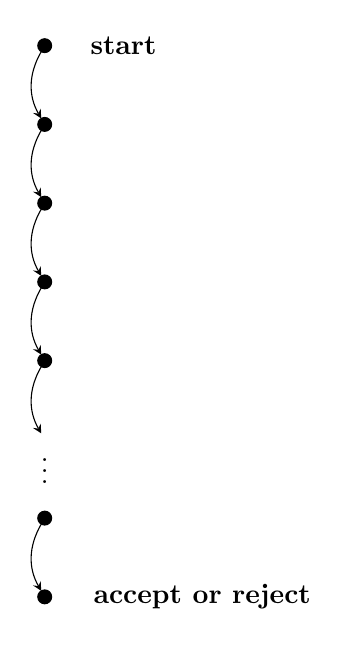
\begin{tikzpicture}[
          auto, >=stealth, node distance=0.0ex and 2em,
          pil/.style={->},
          dot/.style={circle, draw=black, fill=black, minimum size=#1, inner sep=0pt, outer sep=0pt} ]
          %nodes
          \node[dot=5pt, color=black] (start) at (0,10) {};   % start
          \node (s) at (1,10) {\textbf{start}};               % Label start
          \node[dot=5pt, color=black] (v1) at (0,9) {};       % v1
          \node[dot=5pt, color=black] (v2) at (0,8) {};       % v2
          \node[dot=5pt, color=black] (v3) at (0,7) {};       % v3
          \node[dot=5pt, color=black] (v4) at (0,6) {};       % v4
          \node[dot=5pt, color=white] (v5) at (0,5) {};       % v5
          \node (vdots) at (0,4.7) {$\vdots$};
          \node[dot=5pt, color=black] (v6) at (0,4) {};       % v6
          \node[dot=5pt, color=black] (v7) at (0,3) {};       % v7
          \node (a) at (2,3) {\textbf{accept or reject}};  % Label start
          %edges
          \path[pil] (start) edge[bend right] (v1);
          \path[pil] (v1) edge[bend right] (v2);
          \path[pil] (v2) edge[bend right] (v3);
          \path[pil] (v3) edge[bend right] (v4);
          \path[pil] (v4) edge[bend right] (v5);
          \path[pil] (v6) edge[bend right] (v7);
      \end{tikzpicture}
      \caption{Deterministic computation.}
      \label{fig:deterministic}
  \end{subfigure}
  \hspace{5em} % vertical space
  \begin{subfigure}[b]{0.4\textwidth}
    \centering
      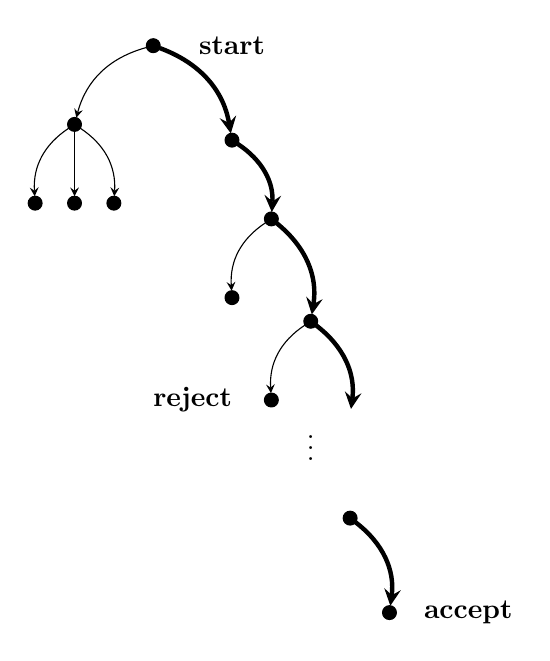
\begin{tikzpicture}[
          auto, >=stealth, node distance=0.0ex and 2em,
          pil/.style={->},
          dot/.style={circle, draw=black, fill=black, minimum size=#1, inner sep=0pt, outer sep=0pt} ]
        %nodes
        \node[dot=5pt, color=black] (start) at (0,10) {};       % start
        \node (s) at (1,10) {\textbf{start}};                   % Label start
        \node[dot=5pt, color=black] (v1) at (-1,9) {};          % v1
        \node[dot=5pt, color=black] (v2) at (1,8.8) {};         % v2
        \node[dot=5pt, color=black] (v3) at (-1.5,8) {};        % v3
        \node[dot=5pt, color=black] (v4) at (-1,8) {};          % v4
        \node[dot=5pt, color=black] (v5) at (-0.5,8) {};        % v5
        \node[dot=5pt, color=black] (v6) at (1.5,7.8) {};       % v6
        \node[dot=5pt, color=black] (v7) at (1,6.8) {};         % v7
        \node[dot=5pt, color=black] (v8) at (2,6.5) {};         % v8
        \node[dot=5pt, color=black] (v9) at (1.5,5.5) {};       % v9
        \node[dot=5pt, color=white] (v10) at (2.5,5.3) {};      % v10
        \node (vdots) at (2,5) {$\vdots$};
        \node[dot=5pt, color=black] (v11) at (2.5,4) {};        % v11
        \node[dot=5pt, color=black] (v12) at (3,2.8) {};        % v12
        \node (a) at (0.5,5.5) {\textbf{reject}};            % Label reject
        \node (b) at (4,2.8) {\textbf{accept}};              % Label accept
        %edges
        \path[pil] (start) edge[bend right] (v1);
        \path[pil, ultra thick] (start) edge[bend left] (v2);
        \path[pil] (v1) edge[bend right] (v3);
        \path[pil] (v1) edge (v4);
        \path[pil] (v1) edge[bend left] (v5);
        \path[pil, ultra thick] (v2) edge[bend left] (v6);
        \path[pil] (v6) edge[bend right] (v7);
        \path[pil, ultra thick] (v6) edge[bend left] (v8);
        \path[pil] (v8) edge[bend right] (v9);
        \path[pil, ultra thick] (v8) edge[bend left] (v10);
        \path[pil, ultra thick] (v11) edge[bend left] (v12);
      \end{tikzpicture}
      \caption{Nondeterministic computation.}
      \label{fig:nondeterministic}
  \end{subfigure}
  \caption{Deterministic and Nondeterministic computations with an accepting branch.}
  \label{fig:computations}
\end{figure}
%%%%%%%%%%%%%%%%%%%%%%%%%%%%%%%%%%%%%%%%%%%%%%%% ENDING OF A FIGURE %%%%%%%%%%%%%%%%%%%%%%%%%%%%%%%%%%%%%%%%%%%%%%%

\subsection{Computational Complexity Classes}\label{subsec:computational-complexity-classes}
Computational complexity theory contemplates not solely the solvability of a problem but also the resources required to solve computational problems.
It is divided in two branches: \textit{Time} complexity and \textit{Space} complexity as mentioned earlier. In this work, we give an informal
description of the classical complexity classes generally encountered. The interested reader can find full details and formal definitions in the
excellent textbook of Sipser \cite{sipserIntroductionTheoryComputation2006}. The following section describes the different computational complexity
classes in which different decision problems fits.

In general, these complexity classes study how the critical resources (\textit{time} and \textit{space}) grows in terms if the input size.
For decision problems, the input is the description of the instance and its size is the number of bits required to encode it.

\subsubsection{Time complexity classes}
We start by characterizing in terms of time. The class $\P$ consists of all problems solvable in polynomial time, that is, all problems solved by
some algorithm in time that is at most linear, quadratic, cubic, or similar in the input size. If $n$ represents the input size, a general polynomial
might look like $5n^{4} + 3n^{2} + 10n - 1$.
Similarly, the class $\EXP$ consists of all problems solvable in exponential time:
$2^{n}, 5^{n}, 2^{n^{2}}$ or in general $2^{p(n)}$ where $p(n)$ is some polynomial. Note that $\EXP$ contains easier problems too, in particular,
all of $\P$.

\subsubsection{Space complexity classes}
On the other hand, the class $\PSPACE$ consists of all problems solvable in polynomial space. This class is the analog of $\P$ but measuring space
instead of time. Similarly, $\EXPSPACE$ consists of all problems solvable in exponential space.

Time and space complexity classes are related in the following way: An optimal algorithm never uses more space than time.
Thus, every problem in $\P$ is also in $\PSPACE$. Also, any (deterministic) algorithm that uses $s$ space can never use more than
exponential-in-$s$ time without repeating a position. Thus, every problem in $\PSPACE$ is also in $\EXP$.

\subsubsection{Nondeterminism}
Next, we consider allowing nondeterminism in order to solve a problem. A nondeterministic algorithm can at any computation step, proceed with
various possibilities (see Fig.~\ref{fig:nondeterministic}). A nondeterministic algorithm can be thought of as an extremely lucky: whenever it needs
to make a decision, it by definition makes the correct choice. The class $\NP$ consists of all problems that can be solved in polynomial time by such a
nondeterministic algorithm. Similarly, we can define $\NPSPACE$ for the nondeterministic analog of $\PSPACE$, and $\NEXP$ for $\EXP$.

\subsubsection{Completeness}
For each complexity class $X$, we call a problem $X$-hard if it is about as hard as every problem in $X$. (Here, we ignore polynomial factors in the
difficulty.) We call a problem $X$-complete if it is both $X$-hard and in $X$. Thus, for example, $\NP$-complete problems are among the hardest problems
in $\NP$, so they must not be in any strictly easier complexity class. Whether $\P = \NP$ is of course a major open problem, but assuming they are even
slightly different, $\NP$-complete problems are not in $\P$. Thus, when classifying a problem into a particular complexity class, showing that the problem
is amongst the hardest problems in a certain complexity class eliminates any doubt of whether the latter belongs in a lower complexity class.
One technique of doing so is by \textit{reduction}.

\paragraph{Reducibility}
By taking a known $X$-complete problem $(B)$ and showing that solving the problem in which we are interested $(A)$ is at least as hard as solving $B$,
we can conclude that $A$ is $X$-hard. We usually do this by showing a way to transform problem $B$ into problem $A$.
\begin{defn}
A function $f : \Sigma^{*} \rightarrow \Sigma^{*}$ is a computable function if on every input $w$, some Turing machine $M$ halts with just $f(w)$ on its tape.
\end{defn}

\begin{defn}
Given two languages $A$ and $B$, $B$ is reducible to $A$ written $B \leq_{p} A$ if there is a computable function $f : \Sigma^{*} \rightarrow \Sigma^{*}$, where for
every $w, w \in B \Longleftrightarrow f(w) \in B$. The function $f$ is called the reduction of $B$ to $A$.
\end{defn}

\subsubsection{Relationship of Complexity Classes} \cite{hearn_demaine_ncl_book}
So far we have that $\P \subseteq \PSPACE \subseteq \EXP$. $\PSPACE = \NPSPACE$ follows from the celebrated result of Savitch \cite{savitch_relationships_1970}.
Concerning nondeterminism, a nondeterministic computation is at least as powerful as regular deterministic computation, so, for example, every problem
in $\P$ is also in $\NP$. On the other hand, nondeterministic computation can be simulated by trying both choices of each decision in turn, which
takes exponentially more time, but about the same amount of space. Thus, for example, every problem in $\NP$ is also in $\PSPACE$. Summing all
together, we can conclude that :
\begin{center}
  $\P \subseteq \NP \subseteq \PSPACE = \NPSPACE \subseteq \EXP \subseteq \NEXP \subseteq \EXPSPACE$
\end{center}
All of the containments are believed to be strict, but beyond the above relations, the only strict containment known among those
classes is $\P  \subsetneq \EXP$. Whether $\P = \NP$ is the most famous unresolved question in Computational Complexity Theory.


\section{Reconfiguration Graph}
Viewing Reconfiguration problems from a graph-theoretic perspective, the notion of a \textit{reconfiguration graph} naturally arises.
Let $G = (V, E)$ be a reconfiguration graph where $V(G)$ is the vertex set consisting of all possible configurations and two nodes are
connected by an edge if the corresponding configurations can each be obtained from the other by the application of a single transformation rule,
\textit{a reconfiguration step}. Any path or walk in the reconfiguration graph corresponds to a sequence of reconfiguration steps called a
\textit{reconfiguration sequence}. Although the terminology concerning reconfiguration problems has not yet stabilized in the litterature those are
the terms that will be used throughout this work.


